\section{Optimisation for Processor Architectures
\label{sec:pa}}

\subsection{NVIDIA GPU}
The LFRic-microbenchmark suite~\cite{lfric-microbenchmarks} allows
optimisations for individual kernels to be explored without having to
compile and run the whole code. This is particularly useful when
targeting a programming model such as OpenACC for GPU architecture
where the Portland group compiler cannot compile the Fortran 2003 of
the whole code.

The local matrix assembly (LMA) matrix-vector kernel had been
previously ported to run on GPUs by inserting OpenACC directives in
the PSy layer code to control the data transfer from host memory to
device memory and to offload the kernel call to the GPU device. This
Open ACC version was the starting point for Alan Gray from NVIDIA to
to look at optimisations. This is a summary of potential optimisations
from NVIDIA.

\begin{lstlisting}[language=Fortran,caption={Code fragment of original 
    kernel},label={lst:LMA-orig}]
  !$acc loop vector 
  do k = 0, nlayers-1
    lhs_e(:,:) = 0.0_r_def
    ik = (cell-1)*nlayers + k + 1

    do df = 1, ndf1
      do df2 = 1, ndf2
        lhs_e(df,k) = lhs_e(df,k) + & 
          matrix(df,df2,ik)*x(map2(df2)+k)
      end do
    end do

    do df = 1, ndf1
      lhs(map1(df)+k) = lhs(map1(df)+k) + lhs_e(df,k)
    end do

  end do 
  !$
\end{lstlisting}

Shown in listing~\ref{lst:LMA-orig} is a code fragment of the LMA
kernel. It has an Open ACC directive \verb+!$acc loop vector+ before the
outmost $k$ loop, so that each thread in a warp will do different loop
iterations. This code runs on a GPU, but not very efficiently. 

The first optimisation is to fuse the two loops over \verb+ndf1+
(lines 6-11 and 13-15) and replace the array \verb+lhs_e+ with a
scalar. The scalar can stay resident in a register for each thread and
avoids uncessary memory accesses. This optimisation is call loop
fuse. 

\begin{lstlisting}[language=Fortran,caption={Optimised
    kernel},label={lst:LMA-opt}]
  !$acc loop vector collapse(2)
  do k = 0, nlayers-1
    do df = 1, ndf1

      ik = (cell-1)*nlayers + k + 1
      lhs_e_scal = 0.0_r_def

      do df2 = 1, ndf2
         lhs_e_scal = lhs_e_scal + matrix(df,df2,ik)*x(map2(df2)+k)
      end do
      
      !$acc atomic update
      lhs(map1(df)+k) = lhs(map1(df)+k) + lhs_e_scal

    end do
  end do
\end{lstlisting}

\begin{table}
\centering
\begin{tabular}{rc}
Optimisation & time (ms) \\\hline
Original     & $9.45$ \\
Loop fusion  & $5.33$ \\
Loop collapse & $2.68$ \\ 
Inlining      & $0.58$ \\
Single Kernel & $0.32$ \\\hline
\end{tabular}
\end{table}

\begin{figure}
\centering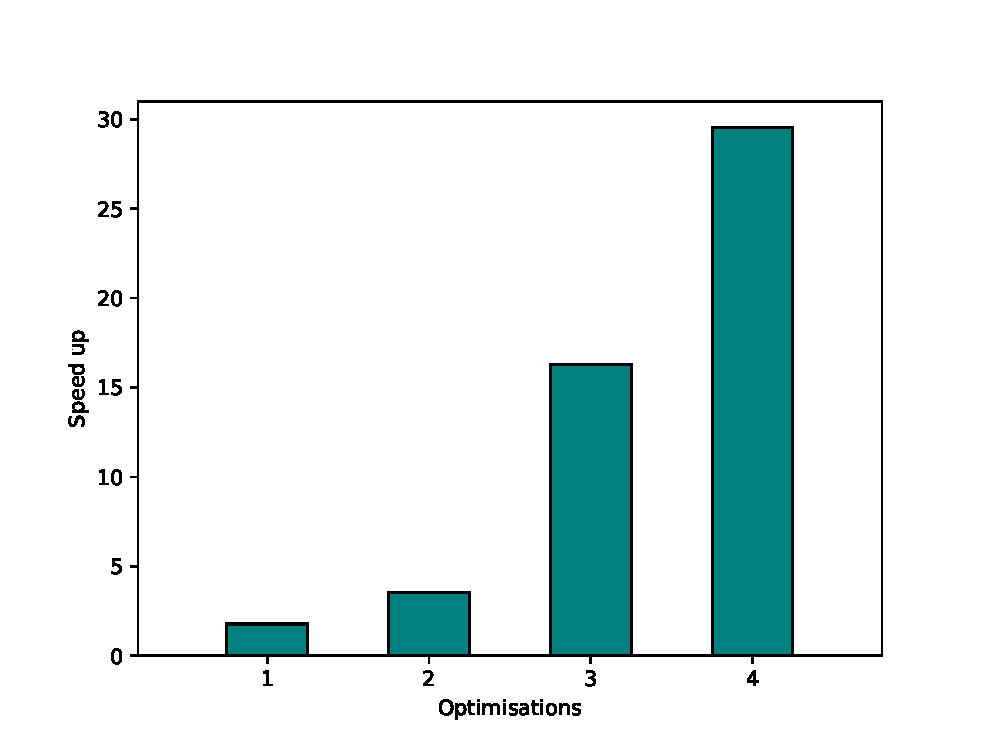
\includegraphics[width=1.0\linewidth]{figs/LMA-nvidia.eps}
\caption{\label{fig:lma_nvidia}Speed up of the LMA kernel against the
  original code for various optimisations. 1 loop fusion. 2 loop
  collapse. 3 Inlining. 4 Single Kernel.}
\end{figure} 



